\subsection{Results}

\subsubsection{GemNet}

\begin{itemize}
    \item s2ef (batch size 2), is2re(batch size 2)
    \item configurations (8 times): baseline stage 0 (all deepspeed features deactivated), 
    stage 0 fp16: memory savings from deepspeed, not only from fp16. 
    \item big drop from stage 0 to stage 1: Optimizer states have huge influence on
    memory consumption, memory-wise, stage 2 with optimizer offloading best
    \item optimizer offloading saves memory, but increases runtime
    \item stage 3 seems ineffective
    \item communication overlapping (pipeline parallelism) seems ineffective.
\end{itemize}

For each experiment, we performed one epoch of training

\begin{figure}[H]
    \centering

    \begin{subfigure}[t]{0.48\textwidth}
        \centering
        \includegraphics[width=\textwidth]{evaluation/gemnet/s2ef/cuda_memory/memory_comparison.pdf}
        \label{fig:gemnet-s2ef-memory-results}
    \end{subfigure}%
    ~
    \begin{subfigure}[t]{0.48\textwidth}
        \centering
        \includegraphics[width=\textwidth]{evaluation/gemnet/s2ef/runtimes/runtimes_comparison.pdf}
        \label{gemnet-s2ef-runtimes-results}
    \end{subfigure}

    \vspace*{-1em}

    \resizebox{0.95\textwidth}{!}{%
    \begin{tabular}{ll|l|l|l|l|l|l|l|l|}
    \cline{3-10}
    & & \scriptsize \textbf{S0}    & \scriptsize \textbf{S0}+fp16 & \scriptsize \textbf{S1}             & \scriptsize \textbf{S1}+OC          & \scriptsize \textbf{S2}+OC & \begin{tabular}{@{}c@{}}\scriptsize\textbf{S2}+OO \vspace*{-0.5em} \\ \scriptsize+OC\end{tabular}      & \scriptsize \textbf{S3}+OC & \scriptsize \begin{tabular}{@{}c@{}}\scriptsize\textbf{S3}+PO \\ \scriptsize+OO+OC\end{tabular} \\ \hline \hline
    \multicolumn{1}{|l|}{\multirow{2}{*}{memory}}   & allocated   & 7.11     & 7.1               & 2.36           & 2.36              & 2.36     & \textbf{1.78} & 3.51     & 2.78              \\ \cline{2-10} 
    \multicolumn{1}{|l|}{}                          & reserved    & 37.71    & 24.98             & \textbf{18.99} & \textbf{18.99}    & 20.3     & 19.77         & 21.99    & 21.32             \\ \hline \hline
    \multicolumn{1}{|l|}{\multirow{5}{*}{runtimes}} & epoch       & 04:07:00 & \textbf{02:29:03} & 02:43:45       & 02:42:51          & 03:00:41 & 04:18:11      & 03:43:01 & 05:09:53          \\ \cline{2-10} 
    \multicolumn{1}{|l|}{}                          & dataloading & 00:00:51 & 00:00:45          & 00:00:29       & 00:00:26          & 00:00:30 & 00:00:29      & 00:00:27 & \textbf{00:00:24} \\ \cline{2-10} 
    \multicolumn{1}{|l|}{}                          & forward     & 00:35:43 & \textbf{00:21:36} & 00:21:59       & 00:21:57          & 00:21:58 & 00:21:57      & 00:54:57 & 00:54:32          \\ \cline{2-10} 
    \multicolumn{1}{|l|}{}                          & backward    & 03:11:31 & 01:53:35          & 01:39:38       & \textbf{01:38:45} & 01:56:29 & 03:09:20      & 02:05:26 & 03:52:43          \\ \cline{2-10} 
    \multicolumn{1}{|l|}{}                          & rest        & 00:18:53 & \textbf{00:13:05} & 00:41:39       & 00:41:41          & 00:41:43 & 00:46:23      & 00:42:11 & 00:22:13          \\ \hline
    \end{tabular}}

    \captionsetup{width=\dimexpr\textwidth-1.5cm\relax}
    \caption{Memory consumption and runtimes on the S2EF task. Memory is in GB, runtimes in the \textit{h:m:s} format.}
    
\end{figure}

\begin{figure}[H]
    \centering

    \begin{subfigure}[t]{0.48\textwidth}
        \centering
        \includegraphics[width=\textwidth]{evaluation/gemnet/is2re/cuda_memory/memory_comparison.pdf}
        \label{fig:gemnet-is2re-memory-results}
    \end{subfigure}%
    ~
    \begin{subfigure}[t]{0.48\textwidth}
        \centering
        \includegraphics[width=\textwidth]{evaluation/gemnet/is2re/runtimes/runtimes_comparison.pdf}
        \label{gemnet-is2re-runtimes-results}
    \end{subfigure}
    
    \vspace*{-1em}

    \resizebox{0.95\textwidth}{!}{%
    \begin{tabular}{ll|l|l|l|l|l|l|l|l|}
    \cline{3-10}
    & & \scriptsize \textbf{S0}    & \scriptsize \textbf{S0}+fp16 & \scriptsize \textbf{S1}             & \scriptsize \textbf{S1}+OC          & \scriptsize \textbf{S2}+OC & \begin{tabular}{@{}c@{}}\scriptsize\textbf{S2}+OO \vspace*{-0.5em} \\ \scriptsize+OC\end{tabular}      & \scriptsize \textbf{S3}+OC & \scriptsize \begin{tabular}{@{}c@{}}\scriptsize\textbf{S3}+PO \\ \scriptsize+OO+OC\end{tabular} \\ \hline \hline
    \multicolumn{1}{|l|}{\multirow{2}{*}{memory}}   & allocated   & 2.88     & 2.88              & 0.62              & 0.62           & 0.62     & \textbf{0.36}  & 1.36              & 1.0         \\ \cline{2-10} 
    \multicolumn{1}{|l|}{}                          & reserved    & 36.27    & 20.6              & \textbf{18.19}    & \textbf{18.19} & 19.24    & \textbf{18.19} & 19.44             & 19.68       \\ \hline \hline
    \multicolumn{1}{|l|}{\multirow{5}{*}{runtimes}} & epoch       & 01:40:32 & 01:03:09          & \textbf{01:01:58} & 01:02:39       & 01:13:23 & 01:33:50       & 01:20:55          & 01:56:20    \\ \cline{2-10} 
    \multicolumn{1}{|l|}{}                          & dataloading & 00:00:09 & 00:00:13          & 00:00:09          & 00:00:09       & 00:00:08 & 00:00:11       & \textbf{00:00:07} & 00:00:15    \\ \cline{2-10} 
    \multicolumn{1}{|l|}{}                          & forward     & 00:24:17 & \textbf{00:15:43} & 00:16:07          & 00:16:06       & 00:16:04 & 00:16:07       & 00:27:31          & 00:27:30    \\ \cline{2-10} 
    \multicolumn{1}{|l|}{}                          & backward    & 01:10:58 & 00:43:16          & \textbf{00:39:29} & 00:39:35       & 00:45:34 & 01:04:43       & 00:42:51          & 01:16:32    \\ \cline{2-10} 
    \multicolumn{1}{|l|}{}                          & rest        & 00:05:07 & \textbf{00:03:55} & 00:06:12          & 00:06:47       & 00:11:35 & 00:12:47       & 00:10:25          & 00:12:01    \\ \hline
    \end{tabular}}

    \captionsetup{width=\dimexpr\textwidth-1.5cm\relax}
    \caption{Memory consumption and runtimes on the IS2RE task. Memory is in GB, runtimes in the \textit{h:m:s} format.}
    
\end{figure}

\subsubsection{DimeNet++}
